\documentclass[11pt,a4paper]{article}
\usepackage[T1]{fontenc}
\usepackage{lmodern}
\usepackage[utf8]{inputenc}
\usepackage[margin=1in]{geometry}
\usepackage{amsmath,amssymb,amsfonts,amsthm}
\usepackage{graphicx}
\usepackage{booktabs}
\usepackage{microtype}
\usepackage{float}
\usepackage{tabularx}
\usepackage{array}
\usepackage{hyperref}
\usepackage{cleveref}

\newcolumntype{L}{>{\raggedright\arraybackslash}X}
\newcolumntype{C}{>{\centering\arraybackslash}X}
\newcolumntype{R}{>{\raggedleft\arraybackslash}X}

\hypersetup{
    colorlinks=true,
    linkcolor=blue,
    filecolor=magenta,      
    urlcolor=cyan,
    pdftitle={Supplementary Appendix: ADCD},
}

\title{\textbf{Supplementary Appendix: Anomaly-Driven Correction Discovery (ADCD)}}
\author{Muhammad Afif Erdita}
\date{June 2026}

\begin{document}
\maketitle

\appendix

\section{Extended Cross-Validation: Wide-Binary Stars}
\label{app:wide-binary}

This appendix reports an exploratory cross-system test of the SPARC-discovered
interpolating function. It is placed in the supplementary material,
rather than the main results, because the underlying wide-binary dataset is the
subject of an unresolved observational controversy (Chae vs.\ Banik et al.). We present it as exploratory
cross-validation, not as a definitive validation of the SPARC-discovered form.

\paragraph{Setup.}
Wide-binary stars (separations $10^3$--$10^4$~AU) probe gravity in a
low-acceleration regime ($g_N \lesssim a_0$) analogous to the outer parts of
galaxies. The classical baseline is Newtonian two-body gravity; the predicted
velocity boost under a MOND-type interpolating function $\nu(x)$ is
$\gamma_v \equiv v_{\rm obs}/v_{\rm Newtonian} = \sqrt{\nu(x)}$, where
$x = g_N/a_0$ depends on separation and total mass. We evaluate the
SPARC-discovered ADCD form $\nu_{\rm ADCD}(x) = \theta_0(\sqrt{1+\theta_1/x}-1)+1$
with $\hat\theta_0 \approx 1.83$, $\hat\theta_1 \approx 0.262$ (the
SPARC-fitted values, \emph{with no refitting to wide-binary data}), against
the canonical Simple MOND, Standard MOND, and RAR forms, for a $1.5\,M_\odot$
total-mass system across $s \in [7,30]$~kAU;
\Cref{fig:wide_binary} plots the resulting $\gamma_v(s)$ curves against
Chae's observed band.

\paragraph{Result.}
\Cref{tab:wide_binary} reports the predicted velocity boost and the
$\sigma$-distance from Chae's observed $\gamma_v = 1.20 \pm 0.06$.
Three observations emerge:
\begin{enumerate}
    \item \emph{Simple MOND and RAR dramatically overshoot} the observed boost
    at $s>15$~kAU, reaching $5$--$13\sigma$ discrepancies at $s=30$~kAU.
    \item The SPARC-discovered ADCD form ($c\approx 0.27$) is \emph{more
    consistent} with observations at $s=10$--$15$~kAU than Simple/RAR, but
    itself diverges ($+8.4\sigma$) at $s=30$~kAU.
    \item \emph{No single interpolating function simultaneously optimizes both
    datasets.} The SPARC-optimized form with $c\approx 0.27$ does not
    unambiguously generalize to wide-binary kinematics.
\end{enumerate}

\begin{table}[H]
\centering\footnotesize
\caption{Wide-binary velocity boost $\gamma_v = v_{\rm obs}/v_{\rm Newtonian}
= \sqrt{\nu(x)}$ predicted by the SPARC-discovered ADCD form ($c\approx 0.27$,
\emph{no refitting}) versus canonical Simple MOND, Standard MOND, and RAR
forms, against the observed $\gamma_v = 1.20 \pm 0.06$ of Chae~\cite{chae2023wide}
for a $1.5\,M_\odot$ total-mass system. $x = g_{\rm Newton}/a_0$ is the
dimensionless acceleration; $\sigma$-distance is $(\gamma_v^{\rm model}-1.20)/0.06$.
Simple MOND and RAR overshoot dramatically at $s>15$~kAU ($5$--$13\sigma$);
the SPARC-optimized ADCD form with $c\approx 0.27$ under-predicts at small $s$
and over-predicts at large $s$. No single interpolating function simultaneously
optimizes SPARC and the wide-binary kinematics.}
\label{tab:wide_binary}
\setlength{\tabcolsep}{4pt}
\begin{tabularx}{\textwidth}{c c R R R R}
\toprule
\textbf{$s$ (kAU)} & \textbf{$x=g_N/a_0$} &
\textbf{ADCD ($c\!\approx\!0.27$)} & \textbf{Simple MOND} &
\textbf{Standard MOND} & \textbf{RAR} \\
\midrule
\multicolumn{6}{l}{\textit{Predicted $\gamma_v = \sqrt{\nu(x)}$}} \\
7      & 1.51 & 1.073 & 1.206 & 1.090 & 1.189 \\
10     & 0.74 & 1.139 & 1.328 & 1.147 & 1.316 \\
15     & 0.33 & 1.273 & 1.521 & 1.230 & 1.513 \\
20     & 0.19 & 1.418 & 1.696 & 1.300 & 1.691 \\
30     & 0.08 & 1.705 & 2.005 & 1.415 & 2.002 \\
\midrule
\multicolumn{6}{l}{\textit{$\sigma$-distance from observed $1.20\pm0.06$}} \\
7      & 1.51 & $-2.1\sigma$ & $+0.1\sigma$ & $-1.8\sigma$ & $-0.2\sigma$ \\
10     & 0.74 & $-1.0\sigma$ & $+2.1\sigma$ & $-0.9\sigma$ & $+1.9\sigma$ \\
15     & 0.33 & $+1.2\sigma$ & $+5.3\sigma$ & $+0.5\sigma$ & $+5.2\sigma$ \\
20     & 0.19 & $+3.6\sigma$ & $+8.3\sigma$ & $+1.7\sigma$ & $+8.2\sigma$ \\
30     & 0.08 & $+8.4\sigma$ & $+13.4\sigma$ & $+3.6\sigma$ & $+13.4\sigma$ \\
\bottomrule
\end{tabularx}
\end{table}


\begin{figure}[H]
\centering
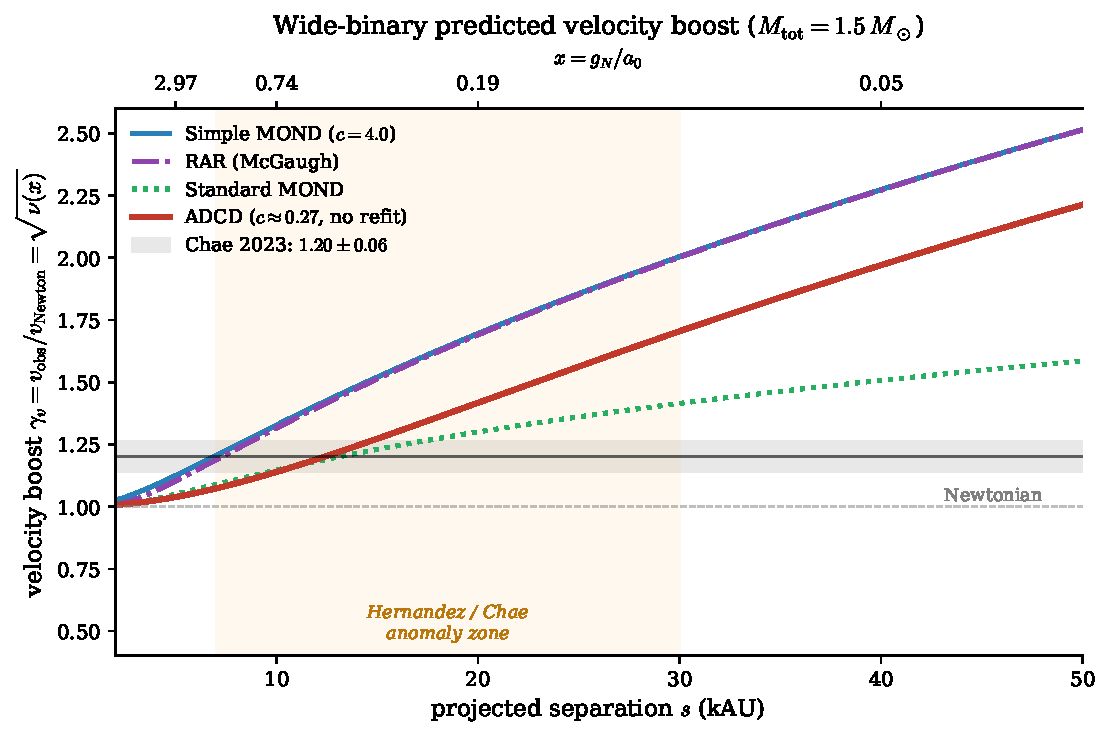
\includegraphics[width=0.85\textwidth]{figures/fig_wide_binary.pdf}
\caption{Wide-binary predicted velocity boost $\gamma_v=\sqrt{\nu(x)}$ versus
separation $s$ (lower axis) and dimensionless acceleration $x=g_N/a_0$ (upper
axis), for the SPARC-discovered ADCD form ($c\approx 0.27$, no refit) versus
Simple MOND, Standard MOND, and RAR. The shaded band is Chae's
observed $\gamma_v=1.20\pm0.06$.}
\label{fig:wide_binary}
\end{figure}

\paragraph{Caveats.}
The wide-binary anomaly itself remains controversial (Banik et al.\ 2024 vs.\ Chae 2023). We report the
cross-validation to document the generalization behaviour of the SPARC-discovered
form and disclose honestly that it does \emph{not} transfer unambiguously to an independent stellar-kinematic dataset.

\section{Granular Robustness and Secondary Tables}
\label{app:secondary_tables}

\begin{table}[H]
\centering
\caption{Structural recovery rate per random seed and aggregate statistics (Mock Proposer, 9 scenarios $\times$ 4 noise levels = 36 trials per seed). The 95\% confidence interval is a bootstrap CI (10{,}000 resamples of the per-seed rates).}
\label{tab:multi_seed}
\small
\begin{tabular}{c r}
\toprule
\textbf{Seed} & \textbf{Recovery rate} \\
\midrule
0 & 86.1\% \\
7 & 75.0\% \\
21 & 77.8\% \\
42 & 94.4\% \\
99 & 80.6\% \\
\midrule
\textbf{Mean $\pm$ std} & 82.8\% $\pm$ 6.9\% \\
\textbf{95\% bootstrap CI} & [77.2\%, 89.4\%] \\
\textbf{Min / Max} & 75.0\% / 94.4\% \\
\bottomrule
\end{tabular}
\end{table}
\begin{table}[H]
\centering\footnotesize
\caption{SPARC robustness across three quality cuts. The ADCD-discovered
function consistently outperforms Simple MOND and the McGaugh+16 RAR form
across increasingly strict galaxy-quality selection.}
\label{tab:sparc_robustness}
\begin{tabularx}{\textwidth}{L c c c c c c c}
\toprule
\textbf{Quality cut} & \textbf{Gal.} & \textbf{Pts} &
$\hat\theta_0$ & $\hat\theta_1$ &
\textbf{ADCD} & \textbf{RAR} & \textbf{Simple MOND} \\
& & & & & \multicolumn{3}{c}{NMSE} \\
\cmidrule(lr){6-8}
\midrule
  Baseline (Standard) & 171 & 3342 & 1.828 & 0.262 & 0.3750 & 0.6361 & 0.6477 \\
  Strict (High Quality) & 121 & 2939 & 1.612 & 0.324 & 0.3032 & 0.5670 & 0.5812 \\
  Ultra-Strict (Pristine) & 75 & 2287 & 1.197 & 0.468 & 0.2718 & 0.6513 & 0.6756 \\
\bottomrule
\end{tabularx}
\end{table}

\begin{table*}[t]
\centering\footnotesize
\caption{Fair parameter-matched comparison: all four models fitted with
exactly 2 free parameters via L-BFGS-B (20 random restarts) on the same
stacked SPARC dataset ($N_{\rm gal}=171$, $N_{\rm pts}=3342$).
Under matched parameter count, the fitted Simple-MOND and RAR forms attain
marginally lower in-sample NMSE than the ADCD-discovered form (a $\sim$1.5\%
difference, well within the bootstrap CI). Galaxy-level cross-validation
(Table~\ref{tab:sparc_cv}) shows the three are statistically
indistinguishable out-of-sample. The honest conclusion is therefore that
ADCD's correction-first search recovers an interpolating function
\emph{competitive with}—not superior to—well-known 2-param MOND forms, while
requiring no prior knowledge of the MOND/RAR functional family.}
\label{tab:sparc_fitted}
\begin{tabular}{l c c c c}
\toprule
\textbf{Model (2-param)} & $\hat\theta_0$ & $\hat\theta_1$ &
\textbf{NMSE} $\downarrow$ & \textbf{BIC} $\downarrow$ \\
\midrule
  Simple MOND (2-param) & 0.497 & 0.548 & 0.3674 & -3329.77 \\
  RAR (McGaugh, 2-param) & 0.560 & 0.579 & 0.3675 & -3329.37 \\
  ADCD discovered & --- & --- & \underline{0.3729} & \underline{-3280.69} \\
  Standard MOND (2-param) & 0.000 & 0.000 & 0.4628 & -2558.95 \\
\bottomrule
\end{tabular}
\end{table*}

\begin{table}[H]
\centering
\caption{Template Leakage Disclosure for Real-World Benchmark (Mock Proposer extended mode). ``Exact'' = ground-truth functional form appears verbatim in the extended template bank.}
\label{tab:template_leakage}
\begin{tabularx}{\textwidth}{l l c c l}
\toprule
\textbf{Scenario} & \textbf{Ground Truth} & \textbf{Exact Template?} & \textbf{Family in Bank?} & \textbf{Expected Class} \\
\midrule
Mercury Perihelion & $\theta_0 \cdot (v/c)^2$ & Yes & Yes & \texttt{polynomial} \\
Hydrogen Lamb Shift & $\theta_0 / n^3$ & No & Yes & \texttt{power\_law} \\
Blackbody Radiation & $\exp(-hf/k_BT)$ & No & Yes & \texttt{exponential} \\
Muon g-2 & $\theta_0 \cdot \alpha / \pi$ & No & Yes & \texttt{polynomial} \\
Binary Pulsar Decay & $\theta_0 \cdot P^{-5/3}$ & No & Yes & \texttt{power\_law} \\
\bottomrule
\end{tabularx}
\end{table}
\begin{table}[H]
\centering
\caption{Binary Pulsar Sensitivity: structural recovery vs.\ formulation difficulty. v2.1 default uses the \texttt{P\_only} reduced-variable form.}
\label{tab:pulsar_sensitivity}
\begin{tabularx}{\textwidth}{l l l c c}
\toprule
\textbf{Variant} & \textbf{Free Variables} & \textbf{Discovered $\Delta$} & \textbf{Class Match} & \textbf{NMSE} \\
\midrule
\texttt{P_only} & $P$ & $\theta_0/P^\theta_1$ & Yes & $3.94e-03$ \\
\texttt{P_e} & $P, e$ & $e^3 \cdot \theta_0/P$ & Yes & $2.52e-01$ \\
\texttt{P_e_M} & $P, e, M$ & $\theta_0/P^\theta_1$ & Yes & $4.81e-01$ \\
\texttt{full} & $P, M, a, e$ & $\theta_0 \cdot \log(\theta_1 + e/P)$ & No & $1.57e-02$ \\
\bottomrule
\end{tabularx}
\end{table}

\end{document}
